\renewcommand{\theequation}{\theenumi}
\begin{enumerate}[label=\arabic*.,ref=\thesubsection.\theenumi]
\item Find the radius and the coordinates of the centre of each of the following circles:
\begin{enumerate}
\item
$
3\vec{x}^T\vec{x}+\myvec{-12 & 6}\vec{x} + 11 = 0
%3x^2+3y^2-12x+6y+11 = 0
$
\\
\solution

The general equation of circle can be expressed as
\begin{align}
    \vec{x}^T\vec{x}-2\vec{c}^T\vec{x}+f = 0\label{eq:solutions/4/1/1/a/eq:1}
\end{align}
where $\vec{c}$ is the centre of the circle and radius of the circle is given as
\begin{align}
r = \sqrt{\norm{\vec{c}}^2 - f}\label{eq:solutions/4/1/1/a/eq:2}
\end{align}
Given equation is
\begin{align}
3\vec{x}^T\vec{x}+\myvec{-12 & 6}\vec{x}+ 11 = 0\\
\vec{x}^T\vec{x}+\myvec{-4 & 2}\vec{x}+ \frac{11}{3} = 0\\
\vec{x}^T\vec{x}-2\myvec{2 & -1}\vec{x}+ \frac{11}{3} = 0\label{eq:solutions/4/1/1/a/eq:3}
\end{align}
Compare Eq \eqref{eq:solutions/4/1/1/a/eq:1} and Eq \eqref{eq:solutions/4/1/1/a/eq:3}
\begin{align}
\implies\vec{c}^{T} = \myvec{2 & -1}\\
\implies\vec{c} = \myvec{2 \\ -1}\label{eq:solutions/4/1/1/a/eq:4}\\
f = \frac{11}{3}
\end{align}
From Eq \eqref{eq:solutions/4/1/1/a/eq:2},
\begin{align}
    \implies r=\sqrt{\brak{2^2 + \brak{-1}^2} - \frac{11}{3}}\\
    = \sqrt{4 + 1 - \frac{11}{3}}\\
    = \sqrt{\frac{4}{3}}\label{eq:solutions/4/1/1/a/eq:5}
\end{align}
From Eq \eqref{eq:solutions/4/1/1/a/eq:4} and Eq \eqref{eq:solutions/4/1/1/a/eq:5}
\begin{align}
   \vec{c} = \myvec{2 \\ -1}\\
    r = \sqrt{\frac{4}{3}}
\end{align}
\begin{figure}[!ht]
\centering
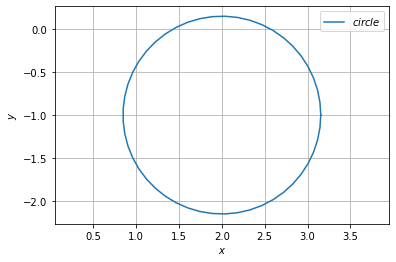
\includegraphics[width=\columnwidth]{./solutions/4/1/1/a/A4.png}
\caption{Circle with radius 1.154 and center coordinates (2,-1)}
\label{eq:solutions/4/1/1/a/Fig:1}
\end{figure}

\item
$
\vec{x}^T\vec{x} = a^2+b^2
$
\item
\begin{align}
  2\vec{x}^T\vec{x}+\myvec{16&-4}\vec{x}+33 = 0 \label{eq:solutions/4/1/1/c/eq1}
\end{align}
\\
\solution

The general equation of a circle is given by
\begin{align}
  \vec{x}^T\vec{x}-2\vec{c}^T\vec{x}+f = 0 \label{eq:solutions/4/1/1/c/eq2}
\end{align}
where $\vec{c}$ is the centre of the circle and r = $\sqrt{\norm{\vec{c}}^2-f}$ is the radius of the circle.
Dividing \eqref{eq:solutions/4/1/1/c/eq1} by 2 and rearranging terms \eqref{eq:solutions/4/1/1/c/eq1} can be rewritten as 
\begin{align}
  \vec{x}^T\vec{x}-2\myvec{-4\\1}^T\vec{x}+\frac{33}{2} = 0 \label{eq:solutions/4/1/1/c/eq3}
\end{align}
Comparing \eqref{eq:solutions/4/1/1/c/eq2} and \eqref{eq:solutions/4/1/1/c/eq3} we get
\begin{align}
  &\vec{c} = \myvec{-4\\1}\\
  &f = \frac{33}{2}
\end{align}
Then centre of the circle \eqref{eq:solutions/4/1/1/c/eq1} is $\vec{c}$ = $\myvec{-4\\1}$ and radius
\begin{align}
  r &= \sqrt{\norm{\vec{c}}^2-f}\\
  &= \sqrt{(-4)^2+1^2-\frac{33}{2}}\\
  &= \sqrt{\frac{1}{2}}\\
  &= 0.7071
\end{align}
  \begin{figure}[!ht]
	\centering
	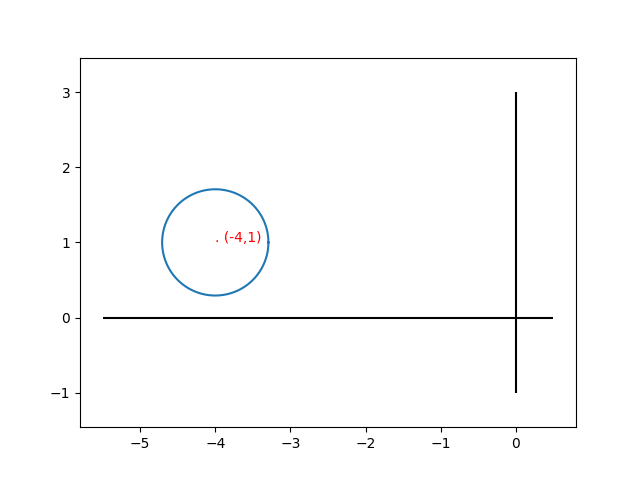
\includegraphics[width=\columnwidth]{./solutions/4/1/1/c/circle.png}
	\caption{Graph of $2x^2+2y^2+16x-4y+33=0$}
	\label{eq:solutions/4/1/1/c/myfig}
\end{figure}

\item
$
36\vec{x}^T\vec{x}-\myvec{36 & 24}\vec{x}-131=0
%36x^2+36y^2-36x-24y-131 = 0
$
\end{enumerate}
\item Find the equation of the circle that passes through the points $\myvec{1\\2}$, $\myvec{2\\1}$, $\myvec{0\\0}$.
\\
\solution
The equation of circle can be expressed as
\begin{align}
    \vec{x}^T\vec{x}-2\vec{c}^T\vec{x}+f = 0
\end{align}
$\vec{c}$ is the centre  and substituting the points in the equation of circle we get
\begin{align}
2\myvec{1&2}\vec{c}-f=5\\
2\myvec{2&1}\vec{c}-f=5\\
2\myvec{0&0}\vec{c}-f=0
\end{align}
can be expressed in matrix form
\begin{align}
\myvec{2&4&-1\\4&2&-1\\0&0&-1}\myvec{\vec{c}\\f} = \myvec{5\\5\\0}
\end{align}
Row reducing the augmented matrix
\begin{align}
\myvec{2&4&-1&5\\4&2&-1&5\\0&0&-1&0}
\xleftrightarrow{R_2\leftarrow 2R_1-R_2}
\myvec{2&4&-1&5\\0&6&-1&5\\0&0&-1&0}\\
\xleftrightarrow[R_1\leftarrow R_1-R_3]{R_2\leftarrow R_2-R_3}
\myvec{2&4&0&5\\0&6&0&5\\0&0&-1&0}\\
\xleftrightarrow{R_1\leftarrow 3R_1-2R_2}
\myvec{6&0&0&5\\0&6&0&5\\0&0&-1&0}
\end{align}
\begin{align}
    \vec{c} = \myvec{\frac{5}{6}\\\frac{5}{6}}\\
    f = 0\\
    r=\sqrt{\norm{\vec{c}}^2-f} = \sqrt{\frac{50}{36}}
\end{align}
The required equation of circle is 
\begin{align}
\vec{x}^T\vec{x}-2\myvec{\frac{5}{6}&\frac{5}{6}}\vec{x} = 0
\end{align}
See Fig. \ref{eq:solutions/4/1/2/Fig1}

\begin{figure}[!ht]
\centering
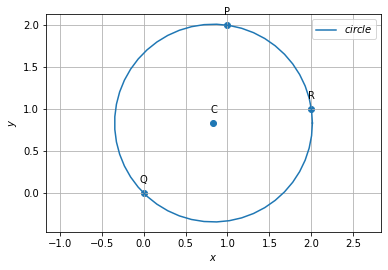
\includegraphics[width=\columnwidth]{./solutions/4/1/2/Circle.png}
\caption{Circle passing through point P,Q,R with centre C.}
\label{eq:solutions/4/1/2/Fig1}
\end{figure}

\item Find the equation of the circle that passes through  the points $\myvec{2\\3}$, $\myvec{3\\2}$, $\myvec{5\\1}$.
\\
\solution
The general equation of circle is represented as
\begin{align}
    \label{eq:solutions/4/1/3/circleeq}
    \vec{x}^T\vec{x}-2\vec{c}^T\vec{x}+f=0
\end{align}
where $\vec{c}$ is the center of the circle. Substituting the given points in the equation \eqref{eq:solutions/4/1/3/circleeq}, we obtain
\begin{align}
    \label{eq:solutions/4/1/3/points}
    2\myvec{2&3}\vec{c}-f=13\\
    2\myvec{3&2}\vec{c}-f=13\\
    2\myvec{5&1}\vec{c}-f=36
\end{align}
can be expressed in matrix form as 
\begin{align}
    \label{eq:solutions/4/1/3/matrix}
    \myvec{4&6&-1\\6&4&-1\\10&2&-1}\myvec{\vec{c}\\f}=\myvec{13\\13\\26}
\end{align}
\begin{figure}[!ht]
\centering
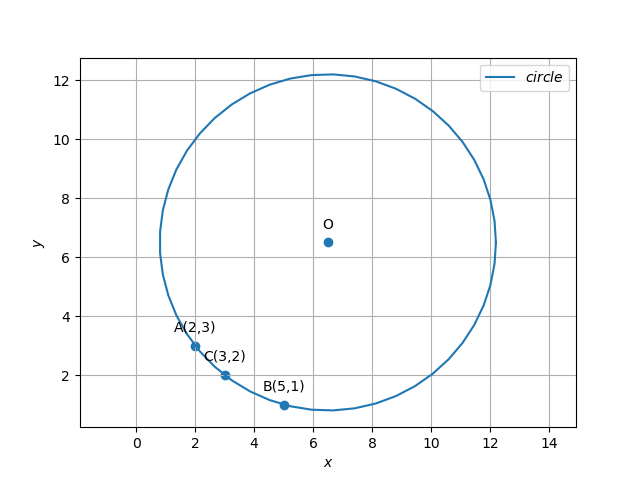
\includegraphics[width=\columnwidth]{./solutions/4/1/3/Circle.png}
\caption{Circle passing through the points A,B,C with center O}
\label{eq:solutions/4/1/3/fig1}
\end{figure}
The augmented matrix for \eqref{eq:solutions/4/1/3/matrix} can be row reduced as follows
\begin{align}
    \myvec{4&6&-1&13\\6&4&-1&13\\10&2&-1&26}\\
    \xleftrightarrow[R_2\leftarrow4R_2-6R_1]{R_3\leftarrow 4R_3-10R_1}
    \myvec{4&6&-1&13\\0&-20&2&-26\\0&-52&6&-26}\\
    \xleftrightarrow[]{R_3\leftarrow 5R_3-13R_2}
    \myvec{4&6&-1&13\\0&-20&2&-26\\0&0&4&208}\\
    \xleftrightarrow[R_1\leftarrow 4R_1+R_3]{R_2\leftarrow 2R_2-R_3}
   \myvec{16&24&0&260\\0&-40&0&-260\\0&0&4&208}\\
   \xleftrightarrow[]{R_1\leftarrow 5R_1+3R_2}
   \myvec{80&0&0&520\\0&-40&0&-260\\0&0&4&208}\\
   \label{eq:solutions/4/1/3/red}
   \xleftrightarrow[R_1\leftarrow \frac{R_1}{40}]{R_2\leftarrow\frac{R_2}{-20},R_3\leftarrow\frac{R_3}{4}}
   \myvec{2&0&0&13\\0&2&0&13\\0&0&1&52}
\end{align}
From the matrix \eqref{eq:solutions/4/1/3/red},
\begin{align}
    \vec{c}=\myvec{\frac{13}{2}\\\frac{13}{2}}\\
    k=52\\
    r=\sqrt{\norm{\vec{c}}^2-f}=11
\end{align}
Hence the circle equation can be written as,
\begin{align}
    \vec{x}^T\vec{x}-2\myvec{\frac{13}{2}&\frac{13}{2}}^T\vec{x}+52=0
\end{align}

\item Find the equation of the circle that passes through the points $\myvec{2a\\0}$, $\myvec{0\\2b}$, $\myvec{a+b\\a+b}$.
\\
\solution
The equation of circle can be expressed as
\begin{align}
    \vec{x}^T\vec{x}-2\vec{c}^T\vec{x}+f = 0
\end{align}
$\vec{c}$ is the centre  and substituting the points in the equation of circle we get
\begin{align}
2\myvec{2a&0}\vec{c}-f=4a^2\\
2\myvec{0&2b}\vec{c}-f=4b^2\\
2\myvec{a+b&a+b}\vec{c}-f=2\brak{a+b}^2
\end{align}
which can be expressed in matrix form
\begin{align}
\myvec{4a&0&-1\\0&4b&-1\\2\brak{a+b}&2\brak{a+b}&-1}\myvec{\vec{c}\\f} = \myvec{4a^2\\4b^2\\2\brak{a+b}^2}
\end{align}
Row reducing the augmented matrix
\begin{align}
\myvec{4a&0&-1&4a^2\\0&4b&-1&4b^2\\2\brak{a+b}&2\brak{a+b}&-1&2\brak{a+b}^2}\\
\xleftrightarrow[R_3\leftarrow R_3-2\brak{a+b}R_1]{R_1\leftarrow \frac{R_1}{4 a}}
\myvec{1 & 0 & - \frac{1}{4 a} & a \\ 0 & 4 b & -1 & 4 b^{2} \\ 0 & 2 \brak{a + b}& \frac{-a + b}{2 a} & 2b\brak{a + b}}\\
\xleftrightarrow[R_2\leftarrow \frac{R_2}{4 b}]{R_3\leftarrow R_3-2\brak{a + b}R_2}
\myvec{1 & 0 & - \frac{1}{4 a} & a \\ 0 & 1 & - \frac{1}{4 b} & b \\ 0 & 0 & \frac{a}{2 b} + \frac{b}{2 a} & 0}\\
\xleftrightarrow[]{R_3\leftarrow \frac{R_3}{\frac{a}{2b} + \frac{b}{2a}}}
\myvec{1 & 0 & - \frac{1}{4 a} & a \\ 0 & 1 & - \frac{1}{4 b} & b \\ 0 & 0 & 1 & 0}\\
\xleftrightarrow[R_1\leftarrow R_1-\brak{-\frac{1}{4 a}}R_3]{R_2\leftarrow R_2-\brak{-\frac{1}{4 b}}R_3}
\myvec{1 & 0 & 0 & a \\ 0 & 1 & 0 & b \\ 0 & 0 & 1 & 0}
\end{align}
\begin{align}
    \vec{c} = \myvec{a\\b}\\
    f = 0\\
    r=\sqrt{\norm{\vec{c}}^2-f} = \sqrt{\brak{a^2+b^2}}
\end{align}
The required equation of circle is 
\begin{align}
\vec{x}^T\vec{x}-2\myvec{a&b}\vec{x} = 0
\end{align}
\begin{figure}[!ht]
\centering
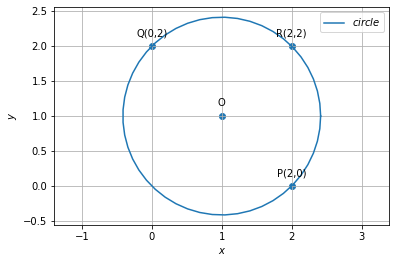
\includegraphics[width=\columnwidth]{./solutions/4/1/4/5.png}
\caption{Circle passing through point P and Q and R}
\label{eq:solutions/4/1/4/Fig:5}
\end{figure}


\item A circle has its centre on the line $x=2y$ and passes through the points $\myvec{-1\\2}$, $\myvec{3\\-2}$.  Find the coordinates
of the centre and the equation of the circle.
\\
\solution
The equation of circle can be expressed as
\begin{align}
    \vec{x}^T\vec{x}-2\vec{c}^T\vec{x}+f = 0
\end{align}
$\vec{c}$ is the centre  and substituting the points in the equation of circle we get
\begin{align}
2\myvec{-1&2}\vec{c}-f=5\\
 2\myvec{3&-2}\vec{c}-f=13\\
\myvec{1&-2}\vec{c}=0
\end{align}
can be expressed in matrix form
\begin{align}
\myvec{1&-2&0\\6&-4&-1\\-2&4&-1}\myvec{\vec{c}\\f} = \myvec{0\\13\\5}
\end{align}
Row reducing the augmented matrix
\begin{align}
\myvec{1&-2&0&0\\6&-4&-1&13\\-2&4&-1&5}
\xleftrightarrow[R_3\leftarrow R_3+2R_1]{R_2\leftarrow R_2-6R_1}
\myvec{1&-2&0&0\\0&8&-1&13\\0&0&-1&5}\\
\xleftrightarrow[R_1\leftarrow R_1+R_2]{R_2\leftarrow R_2/4}
\myvec{1&0&\frac{-1}{4}&\frac{13}{4}\\0&2&\frac{-1}{4}&\frac{13}{4}\\0&0&-1&5}\\
\xleftrightarrow[R_1\leftarrow R_1-R_3/4]{R_2\leftarrow R_2-R_3/4}
\myvec{1&0&0&2\\0&2&0&2\\0&0&-1&5}
\end{align}
\begin{align}
    \vec{c} = \myvec{2\\1}\\
    f = -5\\
    r=\sqrt{\norm{\vec{c}}^2-f} = \sqrt{10}
\end{align}
The required equation of circle is 
\begin{align}
\vec{x}^T\vec{x}-2\myvec{2&1}\vec{x}+5 = 0
\end{align}
See Fig. \ref{Fig:solutions4/1/5/}

\begin{figure}[!ht]
\centering
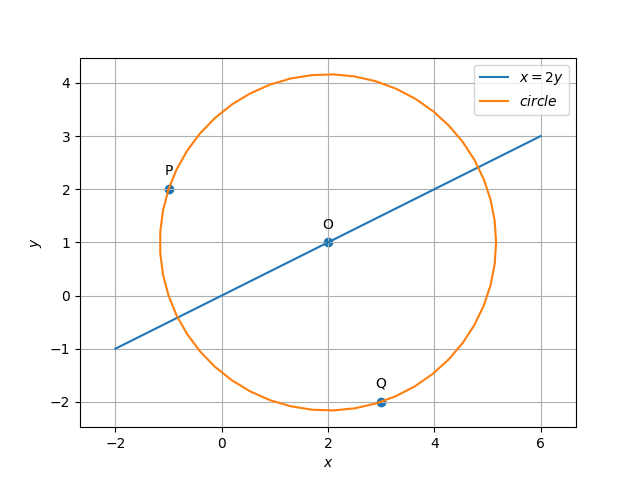
\includegraphics[width=\columnwidth]{./solutions/4/1/5/circle.png}
\caption{Circle passing through point P and Q also centre lie on the line x=2y}
\label{Fig:solutions4/1/5/}
\end{figure}

\item Find the locus of the centre of a circle which touches the line 
\numberwithin{equation}{enumi}
\begin{align}
\myvec{\cos\alpha  & \sin\alpha}\vec{x} =p
\end{align}
 and the circle 
\begin{align}
\norm{\vec{x}-\vec{c}} = r
\end{align}
\end{enumerate}
